\documentclass[titlepage]{article}

\usepackage[letterpaper,margin=1in]{geometry}
\usepackage{fancyhdr}
\usepackage{csquotes}
\usepackage{tikz}
\usepackage{subcaption}

\MakeOuterQuote{"}

\usetikzlibrary{knots}

\newcommand{\dq}[2]{``#1" (#2).}

\title{{\Huge\emph{The Knot Book}}\\[5pt]\textcolor{gray!60!black}{Notes}\vspace{-0.5em}}
\author{Steven Labalme}
\date{\today}

\begin{document}




\pagenumbering{gobble}
\maketitle



\pagenumbering{roman}
\tableofcontents
\listoffigures
\listoftables
\newpage



\pagenumbering{arabic}
\pagestyle{fancy}
\fancyhf{}
\rfoot{Labalme \thepage}
\renewcommand{\headrulewidth}{0pt}
\section{Introduction}
\subsection{Introduction}
\begin{itemize}
    \item \textbf{Knot}: \dq{A knotted loop of string, except that we think of the string as having no thickness, its cross-section being a single point}{2}
    \item Do not distinguish between a `nice, even' knot and one that has been deformed through space.
    \item \textbf{Unknot}: \dq{The simplest knot of all\dots the unknoted circle}{2} \emph{Also known as} \textbf{trivial knot}.
    \item \textbf{Trefoil knot}: \dq{The next simplest knot}{2}
    \begin{figure}[h!]
        \centering
        \begin{subfigure}{0.4\linewidth}
            \centering
            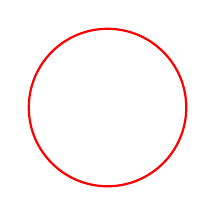
\begin{tikzpicture}
                \draw[red,thick] (0,0) circle (1cm);
            \end{tikzpicture}
            \caption{Trivial knot.}
            \label{fig:circletrefoila}
        \end{subfigure}
        \begin{subfigure}{0.4\linewidth}
            \centering
            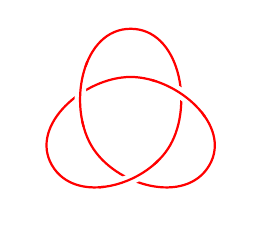
\begin{tikzpicture}
                \begin{knot}[
                    consider self intersections,
                    clip width=5
                ]
                    % could be defined with a combination of polar coordinates and foreach...
                    \strand[red,thick] (1,{3^0.5})
                        to [out=0,in=60] (1.5,0.25)
                        to [out=240,in=-60] (0,0)
                        to [out=120,in=180] (1,1.12)
                        to [out=0,in=60] (2,0)
                        to [out=240,in=-60] (0.5,0.25)
                        to [out=120,in=180] cycle
                    ;
                    \flipcrossings{1,3}
                \end{knot}
            \end{tikzpicture}
            \caption{Trefoil knot.}
            \label{fig:circletrefoilb}
        \end{subfigure}
        \caption{The two simplest knots.}
        \label{fig:circletrefoil}
    \end{figure}
\end{itemize}




\end{document}


% \subsection{Composition of Knots}
% \begin{itemize}
%     \item \dq{hi}{\#\#}
% \end{itemize}


% \subsection{Reidemeister Moves}
% \begin{itemize}
%     \item \dq{hi}{\#\#}
% \end{itemize}


% \subsection{Links}
% \begin{itemize}
%     \item \dq{hi}{\#\#}
% \end{itemize}


% \subsection{Tricolorability}
% \begin{itemize}
%     \item \dq{hi}{\#\#}
% \end{itemize}


% \subsection{Knots and Sticks}
% \begin{itemize}
%     \item \dq{hi}{\#\#}
% \end{itemize}